\subsubsection{Agenten RTE}
Auf der nächsten Hierarchieebene über den Interfaces liegt die Laufzeitumgebung der Agenten (AgentRTE).
\begin{figure}[h!]
	\centering
		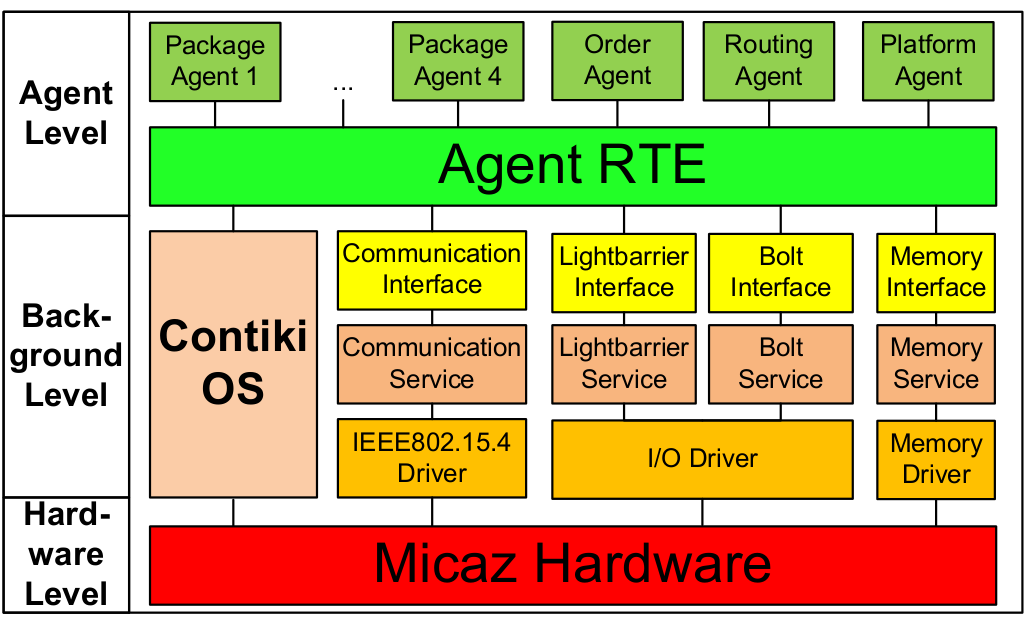
\includegraphics[width=0.9\textwidth]{ArchitekturMicazRampe.png}
	\caption{Architektur Micaz Rampe\cite{Stasch:Hahn}}
	\label{ArchitekturMicazRampe}
\end{figure}
\paragraph{Hardware Level}\mbox{} \\
Auf der Hardwareebene werden die Treiber für die Steuerung der Lichtschranke und Bolzen implementiert. Die Treiber bekommen ein
allgemeines Interface für die Agenten RTE.